%begmin%
	\begin{minipage}{0.6\textwidth}
		
		\item La masa $m$ se encuentra suspendida verticalmente de un resorte de constante el\'astica $k$. El sistema se pone a oscilar de modo que se registra una fuerza de roce $f$ proporcional a la velocidad $v$ dada por la expresi\'on: $f=\sqrt{k m} \ v$.
		
	\end{minipage}
	%\hspace{0.05\textwidth}
	\begin{minipage}{0.4\textwidth}
		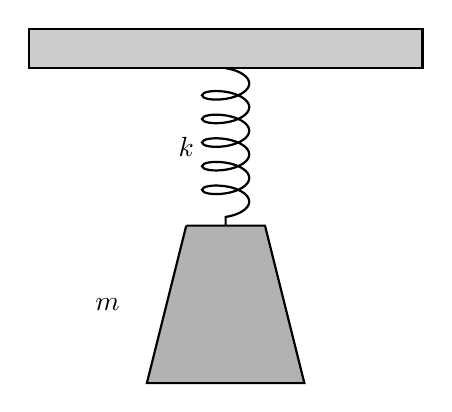
\begin{tikzpicture}
		\filldraw [fill=white!80!black, thick] (-2.5,0)rectangle(2.5,.5);
		\draw [thick, decoration={aspect=0.4, segment length=3mm, amplitude=3mm, coil}, decorate] (0,0)--(0,-2);
		\filldraw [fill=black!30!white, thick] (-.5,-2)--(.5,-2)--(1,-4)--(-1,-4)--(-.5,-2);
		\draw[dotted]
			(-.5,-1) node[scale=1] {\(k\)}
			(-1.5,-3) node[scale=1] {\(m\)}
			;
		\end{tikzpicture}
	\end{minipage}
%endmin%

	\begin{enumerate}[a)]
		\item Deduzca la ecuaci\'on diferencial que describe el movimiento oscilatorio de la masa $m$.

		
		\item Compare el per\'iodo de las oscilaciones amortiguadas con el per\'iodo que se tendr\'ia si el roce fuera despreciable. Determinar la raz\'on entre ambos per\'iodos.
		

		\item Determine la amplitud de las oscilaciones que se conseguir\'ian si se incorpora al sistema una fuerza vertical $F$ sobre $m$ dada por: $F=mg \sin \left( \sqrt{\frac{k}{m}} \ t \right)$		
	\end{enumerate}

\textbf{\underline{Soluci\'on:}}

\begin{enumerate}[a)]
	\item 
	\begin{eqnarray*}
	\sum \vec{F} &=& m \vec{a} \\
	m \ddot{y} &=& -ky - \sqrt{km} \dot{y} + F_{\text{ext}}
	\end{eqnarray*}
	\begin{equation*}
	\ddot{y} + \sqrt{\dfrac{k}{m}}\ \dot{y} + \dfrac{k}{m}y = \dfrac{F_{\text{ext}}}{m}
	\end{equation*}
	
	\item 
	\begin{equation*}
	\omega_0^2 = \dfrac{k}{m} \Longrightarrow T_0 = 2 \pi \sqrt{\dfrac{m}{k}} 
	\end{equation*}
	\begin{equation*}
	\omega_a^2 = \sqrt{\omega_0^2 - \dfrac{b^2}{4m^2}} \text{ , donde } b=\sqrt{km}
	\end{equation*}
	\begin{equation*}
	\omega_a^2 = \sqrt{\dfrac{k}{m} - \dfrac{km}{4m^2}} \Longrightarrow T_a = 2 \pi \sqrt{\dfrac{4m}{3k}}
	\end{equation*}
	\begin{equation*}
	\dfrac{T_a}{T_0} = \dfrac{2 \pi \sqrt{\dfrac{4m}{3k}}}{2 \pi \sqrt{\dfrac{m}{k}}} \Longrightarrow \dfrac{T_a}{T_0} = \sqrt{\dfrac{4}{3}}
	\end{equation*}
	
	\item 
	\begin{equation*}
	\ddot{y} + \sqrt{\dfrac{k}{m}}\ \dot{y} + \dfrac{k}{m}y = g \sin \left( \sqrt{\frac{k}{m}} \ t \right)
	\end{equation*}
	\begin{eqnarray*}
		A_2 &=& \dfrac{F_0}{m} \dfrac{1}{\sqrt{\left( \omega_0^2 - \omega^2\right)^2 + \left( \frac{b}{m} \right)^2 \omega^2 }} \\
		&=& \dfrac{g}{\sqrt{\left( \frac{k}{m} - \frac{3k}{4m} \right)^2 + \frac{k}{m} \frac{3k}{4m} }} \\
		A_2 &=& \dfrac{4}{\sqrt{13}} \dfrac{mg}{k}
	\end{eqnarray*}		
\end{enumerate}